 
This work on using a Gaussian Process for cosmic shear analysis 
was first discussed as a possibility in  \citep{Schneider2014}  and 
forms the basis of the analyses that I helped perform 
in Schneider et al. (in prep.). 

\section{Introduction} 

% why study cosmic shear 
A cornerstone of cosmology is found on the 
observation of the highly Gaussian temperature fluctuations in the cosmic microwave 
background (CMB), an ancient light emitted during the recombination in the early
universe. A number of inflation models can explain how these
nearly Gaussian fluctuations could arise from quantum perturbations in the 
early universe. Furthermore, we know how these perturbations could grow
through linear transfer over time to form a large-scale ($> 10 h^{-1} Mpc$) 
dark matter (DM) density field that is consistent with present
day observables. 
This cosmic web encodes valuable information for constraining cosmological
parameters. Many lensing analyses of the large-scale DM density field, such as from
the Canadian-French-Hawaiian Telescope Lens survey (CFHTLens;
\citealt{Kilbinger2013}), the Deep Lens Survey
(DLS; \citealt{Jee2013a}, \citealt{Wittman2002}), the Dark Energy Survey 
(DES; \citealt{Abbott2016}) and others, 
have already given competitive cosmological constraints for 
 the matter density ($\Omega_m$) and the fluctuation amplitude 
of the matter density ($\sigma_8$) on a particular characteristic scale (8
$h^{-1} Mpc$). 
% The observable, the subtle distortion signals of galaxy shapes 
% that is induced by the gravity of intervening DM
% between far away galaxies and the observers, is also known as cosmic shear.  

% as the Large Synoptic Survey Telescope (LSST) will
% provide data of high enough quality and large enough volume such that the
% constraints will be systematics limited. 
% how complicated is cosmic shear inference 
% have already demonstrated the constraining power  
% constraints.
% This has sparked interests to
% come up with a comprehensive (statistical) framework to address the effects
% from systematics.

% As first discussed in chapter 1, the presence of DM could distort background
% galaxy shapes through gravitational lensing.
The analysis of the gravitational lensing signal from the DM density field, however, is far from trivial. 
The measured distortions in galaxy shapes that reflect the density of intervening DM, 
only provide a weak, indirect shear signal (known as cosmic
shear; $\lensparams$). The signal is also buried among various sources of noise
and systematics. 
To improve the existing constraints, there are many ongoing 
efforts to refine the analysis pipeline. 
In this work, we propose a new approach for representing 
the cosmic shear information and show how it can be used in a probabilistic framework. 
This can allow the joint inference of the signal, the noise and the systematics, 
and potentially provide a less biased estimate of the cosmological parameters 
(${\bf \theta}$). 
The most relevant reference of such a probabilistic approach can be found in 
\cite{Schneider2014} and Schneider et al. (in prep.), 
while an alternative hierarchical approach can be found in \cite{Alsing2015}. 

In general, an analysis framework for cosmic shear includes: \\ 
(1) the identification and deblending of source galaxies from sky survey data 
using software such as {\sc SEXtractor} \citep{Bertin1996}, {\sc Celeste}
\citep{Regier2014}, and / or {\sc Tractor} \citep{Lang2010}, among others;\\
(2) the measurement of the ellipticities of the tracer galaxies  
and the estimation of the measurement error ($\sigma_{\rm
ms}$) via some shape fitting routines; \\
(3) the characterization and correction of atmospheric aberrations and survey masking 
on the shapes of foreground stars using
 a point-spread-function (PSF, which is represented by $\Pi$ in this work; \citealt{Jee2013a}, \citealt{Rowe2010}); \\
(4) the representation of the intrinsic ellipticities of the tracer galaxies by a
distribution, which is usually assumed to be a Gaussian with zero mean
and a variance of $\sigma_e^2 \approx 0.25^2$;\\ 
(5) the estimation of the (photometric) redshift of the source galaxies. The 
estimates of the redshift can be used to weight the lensing kernel
to reflect the different lensing efficiency when the DM overdensities 
are located at different distances from the observer and the source galaxies.
\\
% An alternative use of the redshift is for a tomographic analysis is performed
% to infer the three-dimensional DM density along the line-of-sight;\\
(6) the statistical inference and representation of the cosmic shear signal,
which is the main theme of this chapter;
and finally \\ 
(7) the cosmological simulation efforts for relating all the above contributions to isolate the cosmic shear signal and
estimate the Gaussian part of the DM distribution. 
There is also a non-Gaussian part of the DM distribution that is introduced by processes
such as gravitational collapse. Such a non-Gaussian distribution 
is also inferred from the simulations before    
cosmological constraints are obtained from a fit to a certain representation of
the cosmic shear information. 
% Even though we lay out the different stages of a cosmic shear analysis sequentially,
% performing the analysis separately may introduce unintended biases. This is
% because an estimation or a correction at separate stages may only provide a local
% best fit solution.   

% Even though the representation of the cosmic shear information on constituents
% one step in the entire pipeline, there are a large number of studies that try
% to improve the current methods. Most of the studies make use of summary 
% statistics. 
There are many proposals of how to best represent the cosmic shear information
(step 6). The technical details of each method differ, but most of them use
an estimator that provides a summary of the data.
Examples of commonly used estimators include, the two-point correlation function 
(2PCF) and the corresponding power spectrum, which is part of the Fourier transform of the 2PCF; 
the ring statistics; the aperture mass dispersion; the peak statistics and
their variations. Detailed discussions of each of these can be found in 
\cite{Kilbinger2015} and \cite{Bartelmann2001a}.
An important concern for computing the summary statistics of the cosmic shear 
comes from the lensing physics. As the lensing observables are the second derivatives of the
scalar potential under the Born approximation, we expect them to be curl-free.
In analogy with the electric field, this curl-free part is called the E mode, 
while any divergence-free part due to systematics or second-order effects is called the 
B mode.
An ideal representation of the
cosmic shear, therefore should allow a complete separation of the E-mode and the B-mode.
However, various causes can
introduce B-mode signals to the observed cosmic shear signal. A well-known
cause of mode mixing is known as the finite-interval problem. It is due to
imperfect observation conditions, such as the blending of galaxies at small scales,
or limitations from survey boundaries at large scales \citep{Kilbinger2013}.  
Specific computational implementation of the summary statistics that bins the 
observed shear can also mix the E and B-modes 
(\citealt{Eifler2010},
\citealt{Becker2013}). Instead of a summary statistic, we provide a new 
{\it statistical model} of cosmic shear that may either provide an alternative
perspective to some of the aforementioned problems, or in the best case
scenario, alleviate the problems. 
 
We will also demonstrate how our method
(step 6) are connected to the other relevant analyses (e.g. steps 2, 3, 4). 
The rest of this chapter will have the following structure, we will \\ 
1) Illustrate the basic properties of the Gaussian Process (GP), the model that we
use to represent the cosmic shear signal.\\ 
2) Show the derivation for incorporating the lensing physics in 
a suitable covariance kernel for a Gaussian Process,  
in the process of describing our method, we will comment on how our method is  
similar or different from other approaches for cosmic shear inference.\\
3) Lay out a hierarchical model for making several mass maps 
with the modified Gaussian Process and show some preliminary results \\ 
4) Discuss the limitations and possible extensions to our method.\\
In no part of the computation of the GP do we explicitly assume a cosmological model. All our
derivations follow from either the lensing physics or our statistical method.   
% Our method provides an alternative from having to use the 2PCF to represent the
% Gaussian portion of the cosmic shear information. 
% Source galaxies provide sparse constraints to probe the matter density along
% the line of sight. 

% how does the signal look like? E-mode ? E-mode?
% Uncorrected systematics can show up in the signal  
%  there is also discussion of the current approaches for
% representing the cosmic shear signal.
% There are current approach for representing  
% As we have demonstrated 
% Although our proposed method is only one of the many stages needed for accurate 
% cosmic shear inference, we try to put our method into context by providing two
% basic analyses. The examples will show how our method are related to other
% stages of the analyses (e.g. 2, 3, 4 and 7). 

\section{Method}

% The crucial ingredient for describing cosmic shear is the deterministic
% lensing physics. However, 
% the choice of the representation of cosmic shear affects both the
% inference procedure and the estimation of cosmological parameters. 

\subsection{The basics of a Gaussian Process (GP)}
A Gaussian Process is one of the most studied and published 
generative statistical model for non-parametric regression. 
It allows the inference of the joint probability density 
function (PDF) to describe a set of data. 
While we focus our analyses on how the GP can be utilized to compute a prior
probability for cosmic shear inference, a GP can be extended to 
allow a variety of other uses. In Astronomy, a GP has been used for modeling 
the light curve of exoplanet transits from discrete data points
\citep{Ambikasaran2014a}. A GP can also be used as a prior probability for optimizing the 
model parameters of neural networks \citep{Snoek2012}, in addition to 
other classification, dimensionality reduction 
and pattern extraction tasks
(\citealt{Wilson2013}, \citealt{Duvenaud2013}, \citealt{Rasmussen2006}).
 
It is helpful to understand the mathematical formulation of a GP, 
before discussing how we can adapt the GP to model the lensing observables. 
In a nutshell, a GP smooths the input data using a non-parametric kernel
\citep{Hastie1990} to map the features to a set of predictions. 
We characterize how goodness of fit using a loss function called the log
marginal likelihood. Other popular loss functions in Astronomy and Cosmology 
are the posterior, or the $\chi^2$ function.
% A statistical (or machine learning) model can be any mathematical or stochastic
% function that maps the inputs $\xv$ to the outputs $\psi$. 
% We can quantify how good the mapping is by a loss function to characterize the
% difference between the
% predicted output and the actual outputs. For example, a loss function can be the log
% marginal likelihood, the posterior, or the
% $\chi^2$ function which is commonly used by physicists. 
% There is no unique form of a loss function, a loss function
% should be designed according to the purpose of the analysis.

A GP is the generalization of a multivariate Gaussian 
to infinite dimension \citep{Rasmussen2006}. While a multivariate Gaussian is
specified by a mean vector $\mu$ and a covariance matrix $\Sigma$, 
a GP is specified by a mean vector function $m(\xv)$ and a
covariance kernel function $\kerngp(\xv, \yv)$, based on some input spatial or
temporal coordinates $\xv$. 
By definition, the (spatial) variable $\psi$ described by a GP has a joint distribution of:
\begin{equation}
	[\psi_1, \psi_2, \ldots, \psi_m ]^T \sim \mathcal{N}(m(\xv),
	\kerngp(\xv, \yv)),\label{eq:GP_joint_distribution}
\end{equation}
where $\mathcal{N}$ is a multivariate Gaussian {\it distribution}.
In our case, the vector $\xv$ (and the
notation $\yv$ that is used interchangeably) denotes the
two-dimensional spatial coordinates of $\ngal$ source galaxy locations. 
For a multivariate Gaussian model of $\xv$, 
its dimensionality is given by the number of features of $\xv$.
When $\xv$ that has two spatial coordinates for each observation, 
a corresponding multivariate Gaussian model also has 2 dimensions, 
i.e. the length of $\mu$ and $\Sigma$ are 2 and $2 \times 2$ respectively. 
However, this is not the case for a GP model of $\xv$. 
The mean vector function of a GP $m(\xv)$ is of length $\ngal$, 
whereas the covariance kernel function $\kerngp(\xv, \yv)$
gives a $\ngal \times \ngal$ matrix as its output.
Note that the GP covariance kernel function does not restrict the 
observed length of $\ngal$, and is capable of predicting the values at
unobserved locations $\xv'$, thus the inventors of the GP 
have said that a GP has infinite dimension \citep{Rasmussen2006}. 
In this work, we will refer to the covariance kernel function with one of 
the following names interchangeably, such as the 
covariance kernel matrix, the kernel, the covariance
function or the covariance matrix. 

When the input data $\xv$ is mean subtracted, the covariance function  
completely specifies the GP. 
We first talk about kernels that depend on the data. These types of kernels 
usually consist of a distance matrix. It measures  
how different or similar $\psi$ are at different spatial coordinates $\xv$. 
% In our case, we are interested in
% modeling the spatial fields of the lensing observables $\lensparams\equiv 
% [\kappa, \gamma_1, \gamma_2]$
% at locations $\xv$. The spatial fields $[\kappa, \gamma_1, \gamma_2]$ 
% are the convergence and the two components of shear.
One possible distance {\it matrix} computed using a diagonal metric is: 
\begin{equation}
	r_{i, j}^2 \equiv (\xv_i - \yv_j) (\xv_i - \yv_j), 
	\label{eq:distance}
\end{equation}
where $i, j$ represent the $n$-th galaxy.
A commonly used covariance kernel is the exponential squared kernel. There are two
additional parameters that specify the exponential squared kernel $\kerngp$ 
which we call $\gpparams = [\lambda, l^2]$. The parameters quantifies how the
different spatial entries $\psi$ at different distances should relate to one another: 
\begin{equation}
	\kerngp(\xv, \yv;\gpparams) = \lambda^{-1} \exp\left(\frac{-r^2}{2 l^2}\right),
	\label{eqn:exp_sq_kernel}
\end{equation}
and this expression gives a covariance {\it matrix}. By definition, the (mean
subtracted) data described by a  GP has a joint PDF: 
In a simple example, we illustrate how to: \\
1) interpolate some given data with a conditional distribution of
eq. \ref{eq:GP_joint_distribution}
\\
2) interpret the influence of precision parameter $\lambda$ and the correlation
length $l^2$ on the GP predictions. 
We will also illustrate the use of a composite covariance kernel function.
A composite kernel function is computed from a linear combination of the sum and/or the
multiplication of kernels (\citealt{Duvenaud2013}, \citealt{Rasmussen2006}).  
This is because the product of several Gaussian distributions results in another
Gaussian with a covariance matrix that is a sum of the covariance matrices of
original Gaussians.  


% Specifically, the mean vector $m(x)$ is often set to be zero in the
% GP. The data are usually mean-subtracted before fitting a GP.  
\begin{figure}
	\centering
	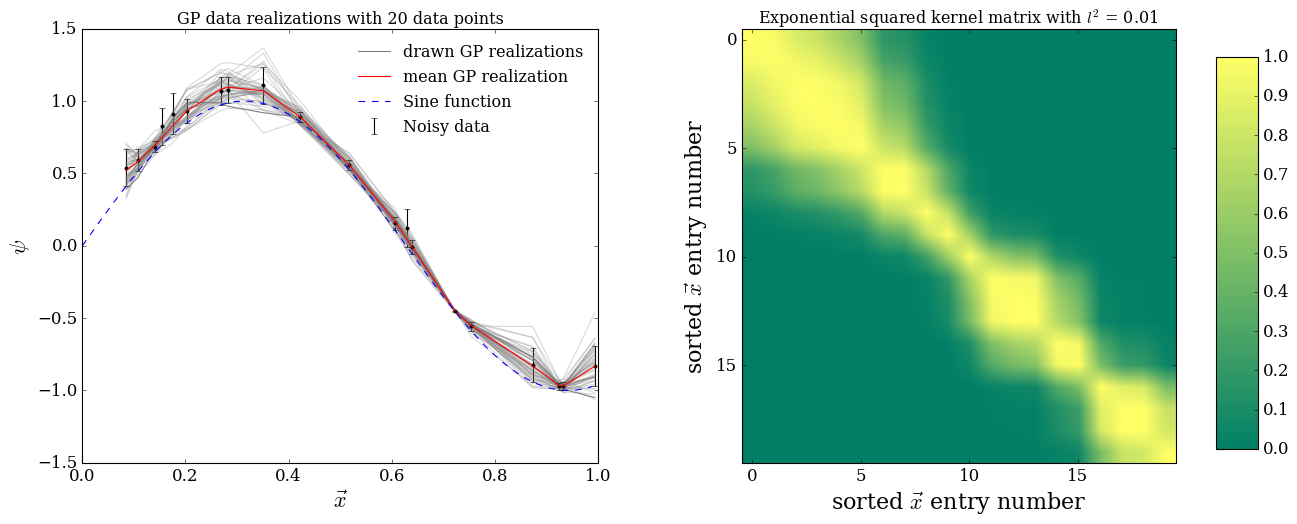
\includegraphics[width=0.9\linewidth]{expSq_kernel_demo_lsq_0pt01.png}
	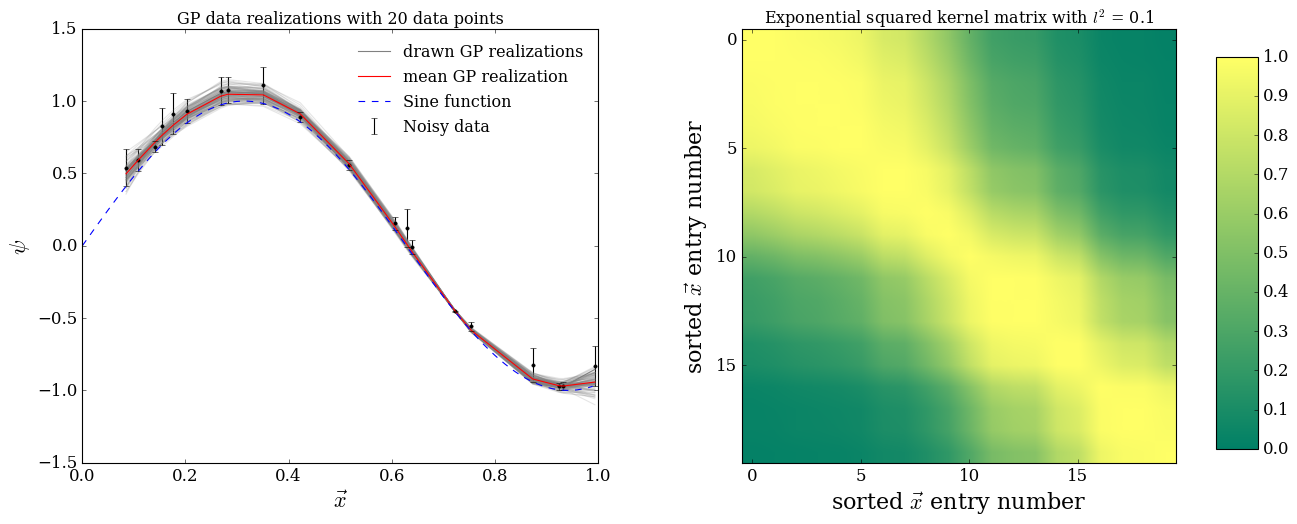
\includegraphics[width=0.9\linewidth]{expSq_kernel_demo_lsq_0pt1.png}
	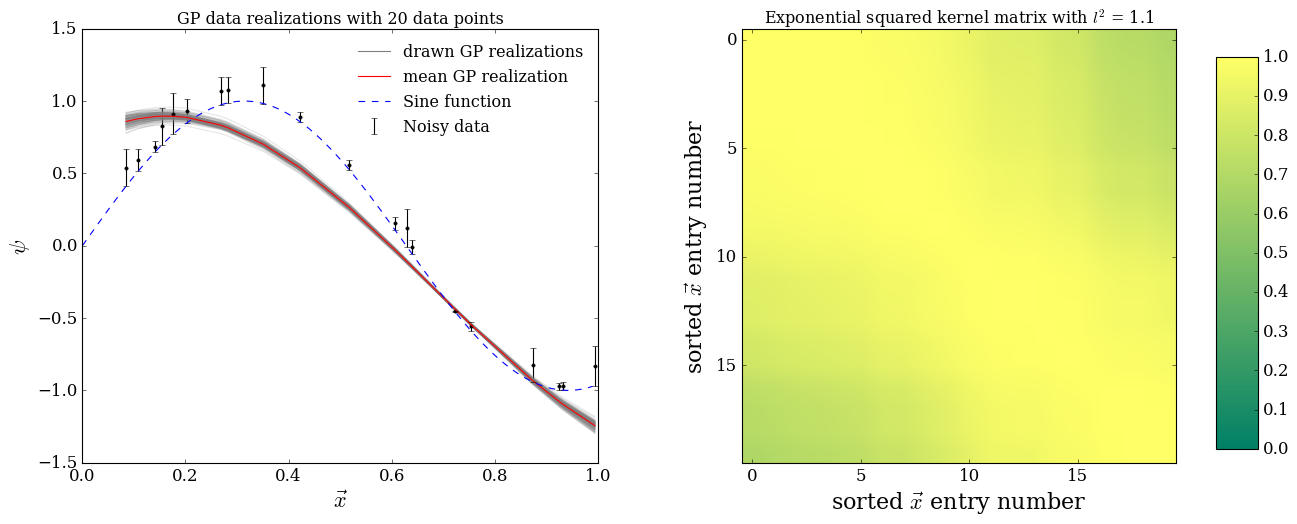
\includegraphics[width=0.9\linewidth]{expSq_kernel_demo_lsq_1pt1.png}
	\caption{
		We show GP models with different correlation lengths (left) and their
		corresponding kernel (right).
		Left: An example GP with a one-dimensional input vector $\xv_\mathds{1}$
		of length 20. The data points (($\psi, \xv_\mathds{1}$); black dots) 
		are generated from a sine function (blue dashed lines).  
		We added some Gaussian noise to the data points as indicated by the error bars. 
		The grey lines indicate the different realizations of
		the predictions given by the corresponding GP, while the red line indicates the
		average of all the realizations.  
		Right: The corresponding exponential squared matrix that is used to model
		the GP on the left. 
		\label{fig:one_d_gaussian_process}}
\end{figure}


\subsubsection{An example: interpolating a set one-dimensional spatial inputs
with a GP}
\label{subsubsec:interpolation}
We illustrate the properties of an exponential squared covariance kernel
$\kerngp$ with a set of one-dimensional spatial inputs $\xv_{\mathds{1}}$. 
This is visualized in Fig. \ref{fig:one_d_gaussian_process}.
% A set of one-dimensional spatial inputs $\xv_\mathds{1}$ can be thought of a set of 
% 2D coordinates along a line.  
% We show the data that we try to model in Fig. \ref{fig:one_d_gaussian_process}.
We draw 20 true data points $\psi_0$ (black points) from a Sine function (blue dashed line) at
$\xv_\mathds{1}$.
We further add Gaussian noise ${\bf\epsilon}$ to the original data $\psi_0$ as
indicated by the individual error bar ($\sigma_i$). 
Given $\xv_\mathds{1}$, we can then compute an exponential squared kernel matrix $\kerngp$ 
by assuming some $\gpparams$ value. Since there is noise
component that are independent and identically distributed (i.i.d) and drawn
from a Gaussian, we can model that using a diagonal noise kernel in the GP kernel. 
The resulting composite kernel is:
\begin{equation}
	\Matrix{K}'_{i, j} = \lambda^{-1} \exp \left(-\frac{r_{i,j}^2}{2 l^2}\right) + \sigma_i^2
	\delta_{i, j}
\end{equation}

In this interpolation problem, we want a way to draw values of $\psi$ from our
model given $\psi_0$. We can do so by computing the conditional distribution of 
$\psi$ given $\psi_0$. Recall the joint distribution of the data
described by a GP is:
\begin{equation}
	Pr(\psi, \psi_0 | \xv) = \mathcal{N}(0, \kerngp') =  \mathcal{N}\left(\left[\begin{array}{c} 0 \\ 0 \end{array} \right], 
	\left(
	\begin{array}{cc}
		A & B \\
		B^T & C
	\end{array}
	\right)
		\right)
\end{equation}
The corresponding conditional distribution can be proven to be \citep{Rasmussen2006}:
\begin{align}
	Pr(\psi | \psi_0, \xv) &= \frac{Pr(\psi, \psi_0 | \xv)}{Pr(\psi_0 | \xv)} \label{eq:conditional_distribution0}\\
	&= \mathcal{N}(BC^{-1}\psi_0, A - BC^{-1}B^T)\label{eq:conditional_distribution}
\end{align}
Note that both the numerator and the denominator are Gaussians in eq.
\ref{eq:conditional_distribution0}. 

In eq. \ref{eq:conditional_distribution}, the multiplication of the different
components of the kernel $\kerngp'$ to
the training points $\psi_0$ allows the kernel to weight $\psi_0$ to compute
the output $\psi$. 
Recall from eq. \ref{eqn:exp_sq_kernel} that 
the precision parameter $\lambda$ affects the 
amplitude of the correlations, while the correlation length (or
the characteristic length scale) $l^2$ 
determines how fast the correlations of  $\psi$ 
fall off across the spatial distance $\xv$. 
The form of exponential squared function creates noticeable structures in the
kernel matrix, i.e. the yellow,
overlapping squares in the top right panel. 
Such structures allow each entry in the output vector $\psi$ to be weighted by
several neighboring spatial entries in $\psi_0$ as a form of smoothing.

As a result of the different correlation lengths for smoothing, 
the predictions fluctuate on specific spatial scales accordingly.
These realizations are represented by the gray lines in the left column of Fig.
\ref{fig:one_d_gaussian_process}. From the top row, we can see that 
the predictions that are drawn from a GP with a small $l^2$ 
fluctuate on a relatively small scale. Even the averaged prediction over
different predicted realizations in the top
left row is not completely smooth. When $l^2$ is increased as we show in the
middle and bottom left panels, we can notice that the predictions are
smoother, but the fit worsens as the $l^2$ value gets too big. In general,  
an optimal set of GP parameters $\gpparams^*$ are found by optimizing the log
marginal (Gaussian) likelihood of a GP.

Another noticeable property of a GP is the probabilistic nature of its predictions
(Fig. \ref{fig:one_d_gaussian_process}).
We can draw many realizations of the predictions to characterize our uncertainty. 
We can compute the 68\% credible levels
by using the minimum and maximum values of 68 out of 100 predictions at each
$\xv$ location.
In such a computation, the credible levels are wider for spatial regions 
with fewer and less certain data points. In the top left panel of Fig.
\ref{fig:one_d_gaussian_process}, we can see that the gray lines can have
larger discrepancies at data point locations $\xv$ with larger error bars, while they
have less discrepancies for data point locations with smaller error bars.

% The probabilistic nature of the GP highlights the main differences of our
% approach vs past analysis approaches. While past analysis computes summary 
% statistics, such as the correlation-function to represent the  
\begin{table}%[htb]
% \small
\begin{center}
\caption{Parameters for our probabilistic model.}
\label{tab:sampling_parameters}
\begin{tabular}{cl}
\hline
Parameter & Description \\
\hline
$\kerngp$ & a general GP covariance kernel {\it matrix}, such as an exponential squared kernel \\
$\kerngp_{\rm GP}$  & the modified GP covariance kernel {\it matrix} that has incorporated
lensing physics\\
${\bf d_{n}}$ & data vector (measured $e_{1,2}$ for each galaxy $n$)  \\
$\sigma_{{\rm ms}; n}$ & ellipticity measurement error for galaxy $n$ 
\\
$\xv$, $\yv$ & vector(s) of 2D spatial locations of galaxies \\
$\epsilon_n^{\rm int}$ & intrinsic galaxy ellipticity for galaxy $n$ \\
$\alpha\equiv\sigma_{e}^2$ & parameters of the distribution of galaxy parameters \\
W & window function for the survey footprint \\
$\lensparams$ & lensing shear and convergence ($\gamma_{1,2}, \kappa$) \\
$\gpparams$ & parameters of the GP kernel\\
% $\rho_{\rm GP}$ & correlation of the GP kernel (element of $\gpparams$) \\
$\lambda$ & precision of the GP kernel (element of $\gpparams$) \\
$l^2$ & squared GP correlation length (element of $\gpparams$) \\
% $\lambda_{\epsilon}$ & precision for the nugget term (element of $\gpparams$) \\
\hline
\end{tabular}
\end{center}
\end{table}


\subsection{Adapting the exponential squared kernel (matrix function) with lensing physics}
There are several families of commonly used covariance kernel.
The ones that are of the highest interest to cosmic shear modeling 
are stationary kernels that can capture 
the homogeneity and the isotropy of the data. This allows the predicted spatial fields
$\psi$ to have properties consistent with the large-scale matter distribution.
%
This kernel matrix $\kerngp(r^2)$ only depends on the
squared magnitude of distances between pairs of galaxy locations. 
This chosen form is, therefore, invariant
under translational and rotational transformations.
% The metric $\Matrix{D}$ is taken to be a diagonal matrix in this discussion but  
% can be generalized to account for anamorphic distortions due to the 
% flat sky approximation. Actual astronomical coordinates uses spherical
% coordinates instead of flat, 2D Euclidean coordinates. 

Additionally, the exponential squared kernel is infinitely differentiable. This
differentiable kernel choice allows us to derive an analytical expression to
relate the different lensing observables to enforce a consistent representation.  
With the use of the Born approximation in the linear regime, the scalar lensing potential $\psi$ is related to 
each of the lensing observables mentioned in chapter 1, e.g. 
$\lensparams \equiv [\kappa, \gamma_1, \gamma_2]$, via the following derivatives:
\begin{align}
\kappa &= \frac{1}{2}\left(\frac{\partial^2 \psi}{\partial x_1^2} +
\frac{\partial^2 \psi}{\partial x_2^2 }\right) 
= \frac{1}{2} (\psi_{,11} + \psi_{,22}),\\ 
\gamma_1 
&=\frac{1}{2}\left(\frac{\partial^2 \psi}{\partial x_1^2} - 
\frac{\partial^2 \psi}{\partial x_2^2}\right) 
= \frac{1}{2} (\psi_{,11} - \psi_{,22}), \\
\gamma_2 
&=\frac{1}{2}\left(\frac{\partial^2 \psi}{\partial x_1 \partial
x_2} + \frac{\partial^2 \psi}{\partial x_2 \partial x_1}\right)
= \frac{1}{2} (\psi_{,12} + \psi_{,21}), 
\end{align}
where we have defined the shorthand for the derivatives of the two spatial dimensions with
subscripts $h,i,j,k = 1, 2$ after a comma.

We show how to derive one of the 6  covariance matrices that we can compute
from $\lensparams = [\kappa, \gamma_1, \gamma_2]$. The computation of the other
covariance kernels is completely analogous.
Since the covariance operator is linear, we can interchange the order of
operation between the covariance operator and the differentiation operators. 
\begin{align*}
&{\rm Cov}_{m,n} (\kappa(\vec{x}), \kappa(\vec{y}))  \\ 
&= \mathbb{E} \left[ 
	(\kappa - \mathbb{E}[\kappa])|_m 
( \kappa - \mathbb{E}[\kappa])|_n\right] 
\\
 &=\mathbb{E}\left[
\frac{1}{2} \left(\frac{\partial^2}{\partial y_1^2} + 
\frac{\partial^2}{\partial y_2^2}\right) 
 (\psi - \mathbb{E}\left[\psi\right])|_n \frac{1}{2}
\left(\frac{\partial^2}{\partial x_1^2} + \frac{\partial^2}{\partial x_2^2} \right)
(\psi - \mathbb{E}\left[\psi\right])|_m \right]
\\
&= \frac{1}{4}\left(
\frac{\partial^2}{\partial x_1^2} \frac{\partial^2}{\partial y_1^2} + 
\frac{\partial^2}{\partial x_1^2} \frac{\partial^2}{\partial y_2^2} +  
\frac{\partial^2}{\partial x_2^2} \frac{\partial^2}{\partial y_1^2} + 
\frac{\partial^2}{\partial x_2^2} \frac{\partial^2}{\partial y_2^2}  
\right) \kerngp_{mn}\\ 
\end{align*}
The resulting 4th derivatives of the covariance
kernels $\kerngp_{\rm GP}$ have the following forms: 
\begin{align}
	\Cov (\kappa(\xv), \kappa(\yv))
&= \frac{1}{4}\left(
\kerngp_{,1111} + \kerngp_{,1122} + \kerngp_{,2211} + \kerngp_{,2222}
\right), \label{eq:kernel_derivatives1}\\
\Cov(\kappa(\xv), \gamma_1(\yv)) &= \frac{1}{4}\left(
\kerngp_{,1111} + \kerngp_{,2211} - \kerngp_{,1122} - \kerngp_{,2222}
\right), \\
\Cov(\kappa(\xv), \gamma_2(\yv)) &= \frac{1}{4}\left(
\kerngp_{,1112} + \kerngp_{,2212} + \kerngp_{,1121} + \kerngp_{,2221}
\right),\\
\Cov(\gamma_1(\xv), \gamma_1(\yv)) &= \frac{1}{4}\left(
\kerngp_{,1111} - \kerngp_{,1122} - \kerngp_{,2211} + \kerngp_{,2222}
\right), \\
\Cov(\gamma_1(\xv), \gamma_2(\yv)) &= \frac{1}{4}\left(
\kerngp_{,1112} + \kerngp_{,1121} - \kerngp_{,2212} - \kerngp_{,2221}
\right), \\
\Cov(\gamma_2(\xv), \gamma_2(\yv)) &= \frac{1}{4}\left(
\kerngp_{,1212} + \kerngp_{,1221} + \kerngp_{,2112} + \kerngp_{,2121}
\right), \label{eq:kernel_derivatives2}
\end{align}
where
\begin{equation}
	\kerngp_{,hijk} = \frac{\partial^4 \kerngp}{\partial x_h \partial x_i
	\partial y_j \partial y_k}.
\end{equation}

With the definition of ${\bf X}_i$ as follows:
\begin{equation}
	\frac{\partial r^2}{\partial \xv_i} = -\frac{\partial
	r^2}{\partial \yv_i} =
	2 \Matrix{D}(\xv - \yv)_i \equiv 2{\bf X}_i,
\end{equation}
we show in Appendix \ref{app:GP_kernel_derivation} 
that each entry $\nu_{,hijk}$ of $\kerngp_{,hijk}$ is
related to each entry $\nu$ of the original exponential squared kernel
$\kerngp$ by:
\begin{equation}
\nu_{,x_h x_i y_j y_k} = (\beta^4 X_h X_i X_j X_k -
\beta^3 (X_h X_i \Matrix{D}_{jk} \delta_{jk} + 5~{\rm perm.}) + \beta^2
(\Matrix{D}_{hj} \Matrix{D}_{ik}\delta_{hj}\delta_{ik} + 2~{\rm perm.})) \nu
\label{eq:4thderivatives}
\end{equation}
with $\beta = l^{-2}$. There are 6 permutations (abbreviated as perm.) of the terms in
eq. \ref{eq:4thderivatives}
multiplied to $\beta^3$ as we can choose two pairs of indices from the $h,i,j,k$ 
when we differentiate the terms by parts, assuming that the order of each
pair of indices matters. 
Likewise, there are 3 possible permutations of
the terms the multiplied to $\beta^2$ as we can choose two pairs of indices from
$h, i, j, k$ where the order of the pairs does not matter.
The derivation of the relevant derivatives and terms are available 
in appendix \ref{app:GP_kernel_derivation} for completeness. 
Our implementation of the GP kernels in eq. \ref{eq:kernel_derivatives1} - 
\ref{eq:kernel_derivatives2} is also openly available at
\href{https://github.com/karenyyng/george}{https://github.com/karenyyng/george}.


\subsection{Making shear predictions (interpolation) with a GP}


\begin{figure}
	\centering
	\includegraphics[width=0.8\linewidth]{gp_cov_v2.png}
	\caption{An illustration of the GP covariance kernel matrix for the {\sc GalSim} data set.
		The same plot is also present in Schneider et al. (in prep.). We can see the various covariance
		and cross-covariance
		structures for the training data $\Upsilon = [\kappa, \gamma_1, \gamma_2]$
		and the interpolated data $\Upsilon' = [\kappa', \gamma_1', \gamma_2']$.
		The spatial inputs in the example are sorted and taken from a line in the
		2D space $\xv$. 
		\label{fig:GP_kernel_vis}}
\end{figure}

Predictions of a GP are made using an appropriate conditional distribution as we have
shown in Section \ref{subsubsec:interpolation}. Although this time instead of a
one-dimensional set of inputs $\xv$, we have 2D coordinates $\xv$ and the
lensing observables are 2D spatial fields.
For predicting lensing observables, our output vector is a concatenation of the
different lensing observables instead, 
\begin{equation}
[\lensparams', \lensparams]  = [\kappa', \gamma_1', \gamma_2', \kappa,
\gamma_1, \gamma_2] 
\end{equation}
The computation of the
conditional distribution mainly follows eq. \ref{eq:conditional_distribution}.
And the partition of the kernel with the modified structure due to eq.
\ref{eq:kernel_derivatives1} to \ref{eq:kernel_derivatives2}
can be see in Fig. \ref{fig:GP_kernel_vis}.
In the presence of shape noise (intrinsic ellipticity) and measurement uncertainties, the actual 
expression of the conditional covariance kernel used for interpolation  
needs two additional white noise kernels.  

Similarly, we can make predictions of $\kappa$ with data from the shear fields. 
Once we can find GP parameters $\gpparams^*$ that optimize the fit to
the observed shear fields $\gamma_{(1, 2)}$ at $\xv$, we can compute $\kerngp_{(\kappa,
\kappa)}$ and draw predictions of $\kappa$ from the conditional distribution. 
Compared with an interpolation method, the mean predictions from a GP are
often more well behaved and do not show drastic increase or decrease 
in the tail regions where there is no data. 
%
Using a GP instead of a summary statistic also allows us to make predictions. 
A prediction model can be any mathematical or numerical function that maps 
the input data to the output appropriately. In the case of a GP, it relies on the covariance
kernel structure to characterize this mapping.  

\subsection{Making mass maps with a GP}
\begin{figure}
	\centering
	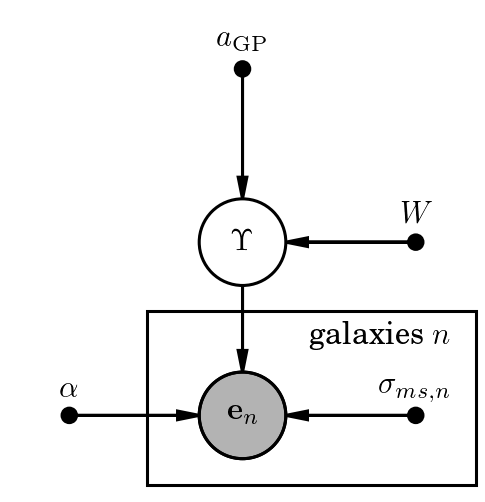
\includegraphics[width=0.4\linewidth]{shear_gp_pgm.png}
	\caption{A simplified probabilistic graphical model (PGM) for inferring
		the lensing observables $\Upsilon$ from survey or simulation data. The dots
		denote fixed parameters in the statistical procedure. The empty circle denotes
		the latent variable, while the shaded circle denotes 
		the observed variable. The plate notation shows the observables that are
		implicitly summed over different galaxies during the computation of matrix-vector
		products in the log marginal likelihood (eq. \ref{eq:log_marginal_likelihood}). The way that the observed
		ellipticity is connected to other branches hints that a joint analysis of
		the connected quantities will provide better predictive performance than if
		they were inferred separately. This figure is also present in Schneider et
		al. (in prep.).
		\label{fig:simplified_pgm}}
\end{figure}

By drawing realizations of the relevant GP, we can compute various 
physical quantities of interest. If the goal is to give the best prediction of a
mass map, it is possible to average over many drawn realizations of the
convergence $\kappa$. And we will show an example of this as a demonstration of
the consistency of our method with other known method for making mass maps.
Or if the shear statistics are of interest, the relevant 2PCF and the power
spectrum can be computed from the mean realization 
after averaging over many realizations of the GP.

\subsubsection{Inferring the optimal GP parameters}
\label{subsubsection:optimize_GP_params}
Throughout the analyses present in this work, 
we make use of the weak shear approximation 
$g = \gamma / (1 - \kappa)  \approx \gamma$, so the observed ellipticity can be
modeled as: 
\begin{equation}
	\epsilon_{(1, 2)} = \epsilon_{\rm int} + g_{(1, 2)}, 
	\label{eq:weak_shear_approx}
\end{equation}
and we can express the contribution of the shape noise $\epsilon_{\rm int}$
and the measurement error
for each galaxy using a composite GP kernel:
\begin{equation}
	\mathsf{S} = \kerngp_{\rm GP} + \sigma_e^2 \mathds{1}  + \sigma_{\rm ms}^2
	\mathds{1}
	\equiv \kerngp_{\rm GP} + \mathsf{N}
	\label{eq:composite_kernel}
\end{equation}
where $\sigma_e^2$ is the variance of the shape noise, and $\sigma_{\rm ms}^2$
represents the measurement error. We can just add the kernels because the
kernels are in the exponential part of the Gaussian function.
Multiplication of Gaussians result in another Gaussian those covariance matrix
is a sum of the covariance matrices of original Gaussians. 
We can then maximize the scalar output of the log marginal likelihood to find the optimal 
$\gpparams^*$: 
\begin{equation}
	\log p(\epsilon_{(1,2)} | \xv) = \frac{-1}{2}\epsilon_{(1,2)}^T \mathsf{S}^{-1}
\epsilon_{(1, 2)}
- \frac{1}{2}\log|\mathsf{S}| - \frac{n}{2}\log(2\pi),
\label{eq:log_marginal_likelihood}
\end{equation}
which consists of a first term that describes the goodness of fit,
and a second term that penalizes complex model assumptions \citep{Rasmussen2006}. 
The complexity penalization term can prevent the GP from overfitting the data.
This allows us to infer a generalizable model for the observed shear, which still
contains contributions from both the shape noise and the measurement
uncertainties. 

\subsubsection{Reconstructing the signal using a Wiener filter}
From our formulation of the observed shear, 
we can reconstruct the noise-free shear signal using a Wiener filter (Wiener 1949). 
The Wiener filter is a linear operator $G$ that transforms the noisy
data to the signal:
\begin{equation}
	G\epsilon_{(1, 2)} = g_{(1, 2)}
\end{equation}
It works by minimizing the expected residual between the estimated signal and the true
signal. This technique has proven successful in the reconstruction of CMB signal
and power spectrum signals (\citealt{Elsner2013} and the references therein).
For signal and noise that are both Gaussian, the Wiener filter gives 
\begin{equation}
	p(\lensparams| \mathbf{d}, \gpparams, \sigma_{\rm ms}, \sigma_e) = \mathcal{N}(\mu_\lensparams,
	\mathsf{S}_\lensparams),
	\label{eq:Wiener_filter_posterior}
\end{equation}
with the data vector being $\mathbf{d} = \epsilon_{(1, 2)}$. We have assumed 
a GP model for the signal as a prior, and we plug in the
optimal GP parameters $\gpparams^*$ obtained from maximizing the log marginal
likelihood for the following quantities derived from the Wiener filter:
\begin{align}
\mu_\lensparams & = \kerngp_{\rm GP}(\kerngp_{\rm GP} + \mathsf{N})^{-1}
\epsilon_{(1, 2)}, \\
\mathsf{S}_\lensparams & = \kerngp_{\rm GP}(\kerngp_{\rm GP} +
\mathsf{N})^{-1}\mathsf{N}.
\end{align}
We use eq. \ref{eq:Wiener_filter_posterior}, which represents the posterior
of our Bayesian model to process two sets of
data for demonstration purposes. A representation of our map-making inference procedure can be seen in Fig. 
\ref{fig:simplified_pgm}. An alternative, but equivalent way of explaining this
model formulation can be found in more detail in Schneider et al. (in prep.).

\subsection{Validation data}
We checked our GP and probabilistic model in eq. \ref{eq:Wiener_filter_posterior}
against one set of synthetic data and one set of real data.
More details about the analysis and the related discussions are in Schneider et 
al. (in prep.).

\subsubsection{{\sc GalSim} data}
The first set of synthetic data that we analyzed was generated via the following procedure: 
We created an angular power spectrum of the convergence signal using {\sc
CHOMP}, a cosmology and halo model code\footnote{A fork of {\sc CHOMP} can be
found at \href{https://github.com/karenyyng/chomp}{https://github.com/karenyyng/chomp}
The original authors of CHOMP are Christopher Morrison, Ryan Scranton and Michael Schneider.
}. 
With the convergence power spectrum, we generated lensed   
galaxy ellipticities using {\sc GalSim}, a modular galaxy image
simulation toolkit \citep{Rowe2015}.
In the process of generating the data, we specified 
the standard Lambda Cold-Dark Matter ($\Lambda$CDM) cosmology with $\Omega_m =
0.3$ and $\sigma_8 = 0.8$, using a narrowly peaked source redshift distribution
at around $z = 1$. As we can specify the intrinsic ellipticity variance
$\sigma_e^2$ from {\sc GalSim}, we made it deliberately small ($\sigma_e^2 =
0.00258$) to speed up our computationally expensive model. 
We also only made use of 1600 source galaxies, each centered on a pixel in a 
$40 \times 40$ grid. 
 
\subsubsection{The Deep Lens Survey (DLS) galaxy cluster Abell 781}
The second set of data was obtained from the DLS, an optical imaging survey 
designed for cosmic shear measurements.  The data points
are centered on the galaxy cluster called Abell 781 in DLS field 2.
There are several previous lensing studies of this cluster, which has an estimated redshift
of $z \approx 0.296$ (\citealt{Wittman2014}, \citealt{Cook2012}, \citealt{Sehgal2008}). 
A galaxy cluster is a
non-linear structure resulted from gravitational collapse. We illustrate that
our GP method can handle non-linear features in the convergence map without 
problem. We selected source galaxies that have photometric redshift $z_b >
0.45$ and with small measurement uncertainties $\sigma_{\rm ms} < 0.1$. We also apply  
a R-band magnitude cut of $22 < R < 23$ and require the ellipticity for the
major (a) and minor axis (b) of the galaxies to satisfy $\sqrt{a^2 + b^2} > 0.8"$ 
to avoid selecting stars. We randomly selected 6000 galaxies that satisfy our
cuts for this analysis. From the selected galaxies, we evaluated the shape
root mean squared amplitude to be $\sim 0.21$, which we take to be the
intrinsic ellipticity scatter $\sigma_e$ in our inference.
Instead of fixing the value, the amplitude
$\sigma_e^2$ can also be inferred with a prior that brackets a reasonable range of
shape noise value.  
 
\section{Results}

\subsection{Validation using simulated data from {\sc GalSim}}
\begin{figure}[!ht]
	\centering
	\includegraphics[width=0.7\linewidth]{mass_map_comparison_galsim.png}
	\caption{A comparison of (right: truth) the maps of the simulated data from {\sc GalSim}  and
	(left: posterior.mean) the maps generated with the use of a GP prior. 
	This figure is a part of Schneider et al. (in prep.). \label{fig:Galsim_massmap}
}
\end{figure}
The mean posterior mass map obtained in Fig. \ref{fig:Galsim_massmap}. 
It shows features that are in general agreement with the true signal. 
It is noteworthy that the resolutions of the posterior maps are coarser ($24 \times 24$
spacing) than the input galaxy
spacing ($40 \times 40$). This reflects how the log marginal likelihood disfavors a sampling
scheme that is higher than the Nyquist frequency. The optimal smoothing length
($l^2 = 0.0123$) from the fitting routine of the log marginal likelihood is also
larger than this Nyquist scale. As we speed up our code to handle a larger
volume and finer
resolution of input data, this limitation from the sampling scheme should
become negligible. We will discuss ways to speed up the computation to enable
the analysis of a denser catalog of data in Section
\ref{subsec:computational_performance}. 

From the averaged posterior map, we also computed the B-mode power spectrum.
The B-mode amplitudes are $< 2e^{-3}$ in the center of the field. 
The B-modes only have larger amplitudes $< 2e^{-2}$ at field boundaries.  
This is expected as \cite{Bunn2003} have shown in a study of the CMB that 
the E and B modes can be mixed when the field of view is incomplete.
Although the B-mode amplitudes from our GP inference are small, 
improvements can be made 
if we understand what GP covariance kernel can represent the B-mode amplitudes to achieve complete E/B mode
separation.

\subsection{Mass mapping for Deep Lens Survey Abell 781}
\begin{figure}[h!]
	\centering
	\includegraphics[width=0.45\linewidth]{kappa_Abell781.png}
	\includegraphics[width=0.45\linewidth]{kappa_Abell781_WD.png}
	\caption{A comparison of mass maps for Abell 781 in the Deep Lens Survey (DLS) 
		\label{fig:Abell781_massmap}.  Left: The smoothed mass (convergence) map of Abell 781 from 
		our GP analysis of 6000 galaxies.
		Right: The higher resolution output generated with $\sim 50000$ galaxies using 
		algorithms from \cite{Wittman2014}. 
		There are five white crosses on each figure showing the locations of X-ray
		peak locations from \cite{Sehgal2008}. No clear mass has been associated
		with the white cross second to the left. 
	These figures are from Schneider et al. (in prep.).
}
\end{figure}
We also see a general agreement of the features in the mass map of Abell 781
(Fig. \ref{fig:Abell781_massmap}) with previous studies of the same cluster 
\cite{Wittman2014}.  
We are restricted by the Nyquist frequency to give a coarser map as discussed
before.   
As the lensing signal from Abell 781 is higher than other fields of the
DLS, we see a better agreement of the inferred $\lensparams$ in field 2 than
other fields. We have not included enough galaxies to allow a good signal and
noise separation for blank fields. 
This is also one of the reasons why  we
 have not inferred cosmological parameters using the
posterior maps of the DLS data.
% We have not inferred the existence of B-mode for the DLS data. 
% There are distortion from stacking exposures (e.g. visible chip gaps features) 
% and other observational limitations (e.g. masking of bright
% stars) that we have not corrected for. 


% Is a non-trivial optimization problem 

\section{Discussion}

\subsection{Relating the lensing observables to a cosmological model}
There is an ongoing effort to explore different ways to relate the posterior lensing signal 
to a cosmological model in Schneider et al. (in prep.). We outline some general
ideas or concerns for such an effort. First, it is possible to use conventional techniques 
 to find the cosmological dependence from simulations.  
We can compute the power spectrum from our mean posterior map. The resulting
power spectrum will have reduced shape noise which may enable direct comparison to
simulations as outlined in previous studies (\citealt{Jee2013a},
\citealt{Semboloni2007}). 
Second, if we were to explore new ways to relate the GP outputs to cosmological constraints,  
it may be interesting to investigate the sensitivity of the GP parameters (and
the covariance kernel models) to cosmological parameters. 
We note that the GP parameters may not be very sensitive to cosmological parameters
due to its flexibility to model a large variety of data. The sampling strategy of
the galaxy locations may also affect the sensitivity. Such a sensitivity test can be
done by repeating our {\sc GalSim} study using convergence power spectrum of different cosmology 
and different sampling. Lastly, if the GP parameters are shown to be
insensitive to cosmological parameters, it is also possible to use dimensionality
techniques to find alternative features in the posterior map that can best determine the
underlying cosmology. 

% \begin{figure}
% 	\centering
% 	\includegraphics[width=0.4\linewidth]{shear_general_pgm.png}
% 	\caption{A more general probabilistic graphical model (pgm) for inferring
% 		the lensing observables $\Upsilon$. The circle denotes
% 		latent variable, while the shaded circle denotes 
% 		the observed variable. The plate notation shows the galaxy entries to sum
% 		over.
% 		\label{fig:general_pgm}}
% \end{figure}

\subsection{The computational performance of the GP}
\label{subsec:computational_performance}
Another big consideration for any cosmic shear inference method is the computational performance.
% As upcoming sky surveys such as the Large Synoptic Survey Telescope (LSST) will
% provide data from billions of source galaxies, 
Any
computationally expensive methods may become infeasible if the algorithm cannot 
analyze enough galaxies to beat cosmic variance. 
% In our case, the computational cost is already an obstacle that keeps us from
% analyzing the entire DLS survey. 
% despite we have a parallelized implementation
% in a fast programming language.   
To achieve high speed performance, we  
implemented the covariance kernels in eq. \ref{eq:kernel_derivatives1} to
\ref{eq:kernel_derivatives2}
in {\sc C++} along with a {\sc Python} wrapper. 
Although the operation of computing and assembling the
derivatives are $O(\ngal^2)$, the large number of addition and 
multiplication operations in eq. \ref{eq:kernel_derivatives1} to
\ref{eq:kernel_derivatives2}, and \ref{eq:4thderivatives} can be slow.
Exploiting the symmetry of the covariance kernel can only provide 
a speed and memory saving of a factor of 2 for the matrix assembly step.

To make the computation run at a reasonable speed, 
I implemented the parallelized computation of each element of the kernel using 
the {\sc OpenMP} library. The slowest step of the entire computation, however, 
is the inversion of the
covariance kernel matrix for the evaluation of the marginal likelihood in eq.
\ref{eq:log_marginal_likelihood}, 
which is an $O(\ngal^3)$ operation. 
I made use of a multi-threaded version of the Cholesky decomposition via the {\sc Intel Math
Kernel Library} to invert the matrix. I achieved a $\sim10$ 
times speedup so the computation and the evaluation of the likelihood of each set of GP parameter
take $\lesssim 3s$ for 1600 galaxies, which translates to 
the inversion of a 4200 $\times$ 4200 covariance matrix.
With the use of distributed computational resources, it is possible 
to probe the space of possible GP parameters by assigning each node to only
evaluate the log marginal likehood for one set of parameters. 
But the scalability of our method is limited by the available memory on each
computer node.

Currently, our method is not as computationally competitive as the 2PCF. 
The fastest implementation of 2PCF has a computational complexity of
$O(n_{\rm gal}\sqrt{n_{\rm gal}})$.
The 2PCF algorithm has also been demonstrated to scale almost linearly with
computational resources 
using a distributed and multi-threaded implementation \citep{Chhugani2012}. 

In terms of speed optimization for our method, rather than relying on 
a parallel computation of the kernel, there are several 
possible approximations that can provide huge speedup. 
Since there are many zero entries in the covariance kernel as shown in
Fig.\ref{fig:GP_kernel_vis}, it may be acceptable to put the kernel in a sparse
computational representation \citep{Snelson2007}. 
Thus, numerical libraries for sparse matrix 
operations (such as {\sc ScaLAPACK} or {\sc PLAPACK})
can provide speedup from looping over fewer data entries. 
An existing field of study that shows how the sparsity
approximation may affect the statistical inference is called covariance tapering. 

On the other hand, there have been successes of further speedup for a GP than
pure sparsity approximations. This requires the introduction of  
 synthetic data sets called inducing points (\citealt{Snelson2006},
\citealt{Rasmussen2006}). Inducing points are latent variables that represent
hidden connections between the training data set and the test set. 
% It relies on fact that the majority of the information content 
%  may be embedded in certain direction (principal components) 
% in the high dimension of the data.
% The large number of data points specifies more about the initial conditions than the
% underlying cosmology.
With the help 
of inducing points,
the inversion of the covariance kernel can be sped up to
$O(M^2 n_{\rm gal})$ for
building the model and $O(M^2)$ for interpolating / predicting output functions
at a new number of inducing data locations M, with M $\ll n_{\rm gal}$ 
\citep{Snelson2006}. While the speedup from inducing point methods is
promising, careful studies need to be done to see how it affects the
inference of cosmological parameters. 
% We note that the vast amount of data
% points in other methods for cosmic shear information may contain more
% information about the initial condition than the cosmological parameters.
  
\subsection{Alternative kernel choice(s) for encoding the lensing physics}
Besides improving the computational performance, the model design of our GP can
also be refined.
Alternative choices for a covariance kernel for describing the lensing physics 
include the family of Mat\'{e}rn kernels:
\begin{equation}
	\kerngp(\xv, \xv') = \frac{1}{\Gamma(\nu)2^{\nu-1}}\left[
		\frac{\sqrt{2\nu}}{l}|\xv - \xv'|
	\right]^\nu K_\nu \left(\frac{\sqrt{2\nu}}{l}|\xv-\xv'|\right) 
\end{equation}
where $K_\nu$ is the modified Bessel function of the second kind, with an order
$\nu$, whereas $l$ is the characteristic length scale.
The smoothness of the data generated from a Mat\'{e}rn kernel is closely
related to the degree of freedom $\nu$ of the kernel. 
The higher degree of freedom it has, the smoother the spatial variations of the
drawn $\psi$ would be for the same characteristic length scale $l$.
Note that a Mat\'{e}rn kernel is also only differentiable to the $(\nu-1/2)$ order.
If we wish to relate our kernels to the lensing potential through the 4th
derivative, we can only use Mat\'{e}rn kernels with $\nu > 9/2$. 
When we take the limit of the degree of freedom of a Mat\'{e}rn kernel to infinity, 
we recover the exponential squared kernel. The inclusion of a Mat\'{e}rn kernel
in addition to an exponential squared kernel, therefore, can pick up features
that are less smooth. The use of an additional Mat\'{e}rn kernel may mitigate the
restrictions from Nyquist sampling but this hypothesis should be verified with
numerical experiments. 

%  The manual differentiation of the analytical form of the kernels can be tedious,
% it may be desirable to generalize the derivation of derivatives. Technologies such
% as automatic differentiation can spreads factors of the derivatives over a tree
% structure to allow almost exact computation. 
 

\subsection{Modeling the systematics and noise via a composite kernel}
Besides kernels that describe homogeneous and isotropic data,
there are other types of periodic kernels that may be useful
in modeling systematics. 
Patterns such as masking or footprints of the telescope due to the
stacking of multiple exposures are obvious during the visualization of the
galaxy density for DLS. 
Previous studies of modeling the PSF
have made use of interpolation with polynomial splines of foreground stars 
for such a task (\citealt{Rowe2010},
\citealt{Jee2013a}).  Instead, a GP can be used to represent the PSF distortions
of foreground stars in a more generalizable way and be
applied as a prior. This allows a probabilistic connection of the noise correction to the rest of the
analysis. The successful examples of noise removal with a GP go beyond 
the aforementioned Wiener filter formulation \citep{Perez-Cruz2013}.

To pick up undetermined periodicity or patterns, 
we can use composite kernels with different covariance structures, 
which can be formed by the addition and/or multiplication of several kernels,
\begin{equation}
	\kerngp = \sum_i \kerngp_i(\gpparams^i).
\end{equation}
By fitting for the best values for $\gpparams^i$, it is possible  
to pick up (sometimes non-obvious) patterns in the data. 
For the best illustration for pattern discovery with a GP, see
\cite{Duvenaud2013}.
It contains a famous example of GP making use of a composite kernel to pick up both the 
short and long term periodic trends for carbon dioxide emission at Mauna Loa.
Additionally, it is physically interesting to examine whether the kernels that best 
fit systematics and incompleteness can represent most of the B-mode components. 

\subsection{Comparison to other representation of shear information}


% - [ ] describe why the lensing observables shouldn't have a B mode 
% Since the lensing observables are the second derivatives of a scalar field,
% it is known that they should be curl free and only contain E-mode signal. 

% It is well known that gravitational lensing, as presented in chapter 1,
% only induces a curl-free (E-mode) shear signal. However, the computation of 
% summary statistics at certain length scale can induce a B-mode (with non-zero
% curl) signal. 

%  \begin{align}
% 	\kappa^E & = \kappa\\
% 	\kappa^B & = 0 \\
% 	\gamma^E &= \left[\frac{1}{2} (\psi^E_{,11} - \psi^E_{,22}) -
% 	\psi^B_{,12}\right]\\
% 	\gamma^B &= \left[\psi^E_{,12} + \frac{1}{2} (\psi^B_{,11} - \psi^B_{,22})\right]
% \end{align}
% Can handle sharp boundaries from stacking images 
% cite Jee2013a  
% cite Rowe2010 paper for interpolating star fields for 
% PSF ellipticity corrections 


\section{Conclusion}
We have derived and implemented a fully probabilistic method for 
representing the lensing observables. By analyzing two sets of data, 
we have demonstrated reasonable agreement between our method and both the true
simulated signal or with past analysis techniques.  
Due to the computational performance restriction,  
the potential of using a Gaussian Process for the inference of cosmological
constraints from outputs of our model remains to be proven. 
If those challenges can be solved with some of our
suggestions, the GP model can be 
extended to provide a joint analysis of the systematics and noise. 


% Requires the understanding of the underlying physical observable, how the statistical
% approach can carry the information and how to actual execute the computation in
% a tractable way.


\section{Acknowledgement}
We thank Chris Paciorek for discussion about the statistical
framework for performing shear inference and the
use of Gaussian Processes.
This research
used the resources of the National Energy Research Scientific 
Computing Center (NERSC), a DOE Office of Science
User Facility supported by 
of the U.S. Department of Energy under Contract No.
DE-AC02-05CH11231.
 This work uses a modified version
of the public code for GP inference {\sc George} available at \href{https://
github.com/karenyyng/george}{https://
github.com/karenyyng/george}, which was forked from \\
\href{https://github.com/dfm/george}{https://github.com/dfm/george}.



